\documentclass{article}
\usepackage{tikz}
\usepackage{tqft}

\begin{document}
\begin{tikzpicture}[every node/.style={tqft/cobordism style={draw,thick,red}}]
 \node[
   tqft,
   fill=orange,
   fill opacity=.5,
   tqft/boundary style={fill=purple},
   tqft/cobordism style={draw,thick,red},
   tqft/boundary lower style={draw,dashed,thick,blue},
   tqft/boundary upper style={draw,green,thick},
   tqft/incoming boundary components=4,
   tqft/outgoing boundary components=6,
   tqft/offset=-1.5,
 ] (a) {};
 \node[pin=north:1] at (a.incoming boundary 1) {};
 \node[pin=north:3] at (a.incoming boundary 3) {};
 \node[pin=south:1] at (a.outgoing boundary 1) {};
 \node[pin=south:4] at (a.outgoing boundary 4) {};
 \node[pin=south:6] at (a.outgoing boundary 6) {};
 \end{tikzpicture}

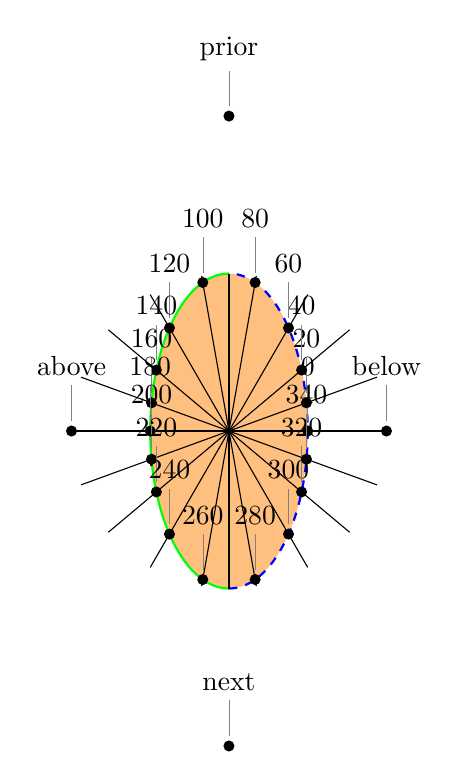
\begin{tikzpicture}[tqft/flow={east},every node/.style={tqft/cobordism style={draw,thick,red}}]
 \node[
   tqft boundary circle,
   tqft/circle width=2cm,
   tqft/circle depth=1cm,
   tqft/boundary separation=4cm,
   fill=orange,
   fill opacity=.5,
   tqft/boundary style={fill=purple},
   tqft/cobordism style={draw,thick,red},
   tqft/boundary lower style={draw,dashed,thick,blue},
   tqft/boundary upper style={draw,green,thick},
   tqft/incoming boundary components=4,
   tqft/outgoing boundary components=6,
   tqft/offset=-1.5,
 ] (a) {};
 \fill (a.next) circle[radius=2pt] node[pin=north:next] {};
 \fill (a.prior) circle[radius=2pt] node[pin=north:prior] {};
 \fill (a.above) circle[radius=2pt] node[pin=north:above] {};
 \fill (a.below) circle[radius=2pt] node[pin=north:below] {};
 \draw (0,0) -- (90:2);
 \draw (0,0) -- (0:2);
 \draw (0,0) -- (180:2);
 \draw (0,0) -- (270:2);
\foreach \ang in {0,20,...,340} {
 \fill (a.\ang) circle[radius=2pt] node[pin=north:\ang] {};
 \draw (0,0) -- (\ang:2);
}
 \end{tikzpicture}

\end{document}